% TAAI 2026 國內論文（中文版）——依 TAAI 2026 國內論文組官方中文 Word 範本修正格式的版本
% 投稿以同目錄 taai2026-domestic-full-paper.docx 為準：該檔直接以官方範本
%   https://taai2026.github.io/assets/downloads/template/taai2026-domestic-full-paper-template-zh.docx
% 的樣式建立，Word 排版為 6 頁。本檔與 .docx 文字相同，版面參數比照範本（A4、上下左右各 2.5 cm、雙欄、
% 內文 10 pt 標楷體＋Times New Roman、單行間距對應範本 18 pt 文件格線、圖表標題置於下方、無頁碼），
% 以 XeLaTeX 編譯；斷行與分頁未必與 Word 相同，投稿前請以 .docx 匯出的 PDF 確認頁數。
% 每一處修訂的原文、原因、修正內容與數據來源，見同目錄〈論文修訂說明.md〉；圖檔在 Image/論文修訂說明/。
% 數據來源（皆為交付版本）：
%   影像辨識：OneLeaf-dx/detection docs/v13_報告_最終交付與週會決議.md、docs/v5.7_報告_交付與研究限制.md、
%             docs/v5.7_結果_兩臂訓練評估.md、weight/best/v13/README.md；
%             Train Code/v11.5/Train_output/extracted/{runs/detect,eval}/v5.7_v11_5/（圖 1、圖 2 由此重繪）
%   端側 RAG：OneLeaf-dx/report 系統測試與評估/20260924_citrus_rag_ablation_study.md（表 1）、
%             系統測試與評估/20260729_mobile_rag_benchmark.md（早期原型執行緒測試）；
%             OneLeaf-dx/citrus-rag-mobile lib/core/services/（檢索、護欄與推論參數）
\documentclass[10pt,twocolumn,a4paper]{article}
\PassOptionsToPackage{no-math}{fontspec}
\usepackage{xeCJK}
\usepackage[a4paper,margin=2.5cm,columnsep=0.75cm]{geometry}
% 範本字型：英數 Times New Roman、中文標楷體（Windows 名稱 DFKai-SB，macOS 名稱 BiauKai）
\IfFontExistsTF{Times New Roman}{\setmainfont{Times New Roman}}{\setmainfont{Tinos}}
\IfFontExistsTF{DFKai-SB}{\setCJKmainfont[AutoFakeBold=2.5,AutoFakeSlant=0.2]{DFKai-SB}}
  {\IfFontExistsTF{BiauKai}{\setCJKmainfont[AutoFakeBold=2.5,AutoFakeSlant=0.2]{BiauKai}}
    {\setCJKmainfont[AutoFakeBold=2.5,AutoFakeSlant=0.2]{AR PL UKai TW}}}
\usepackage{setspace}
\usepackage{graphicx}
\graphicspath{{Image/論文修訂說明/}}
\usepackage{array}
\usepackage{cite}
\usepackage{caption}
\usepackage{titlesec}
\usepackage[hidelinks]{hyperref}

% 單行間距：範本以 18 pt 文件格線排 10 pt 內文
\setstretch{1.5}
\pagestyle{empty}
\setlength{\parindent}{2em}
\setlength{\parskip}{0pt}

% 標題靠左、粗體；第一層 12 pt「1.」，第二層 11 pt「2.1.」
\titleformat{\section}{\normalfont\fontsize{12}{18}\selectfont\bfseries}{\thesection.}{0.5em}{}
\titleformat{\subsection}{\normalfont\fontsize{11}{18}\selectfont\bfseries}{\thesubsection.}{0.5em}{}
\titlespacing*{\section}{0pt}{9pt}{6pt}
\titlespacing*{\subsection}{0pt}{6pt}{3pt}

% 圖表標題：粗體 10 pt，置於圖表下方，形如「圖1.」「表1.」；一行置中、多行靠左
\renewcommand{\figurename}{圖}
\renewcommand{\tablename}{表}
\DeclareCaptionLabelFormat{zhnum}{#1#2.}
\captionsetup{labelformat=zhnum,labelsep=space,font={normalsize,bf},justification=raggedright,singlelinecheck=true,skip=4pt}
\captionsetup[table]{position=below}

% 參考文獻：編號標題、10 pt、12 pt 固定行距
\makeatletter
\renewenvironment{thebibliography}[1]
  {\section{參考文獻}%
   \list{\@biblabel{\@arabic\c@enumiv}}%
        {\settowidth\labelwidth{\@biblabel{#1}}%
         \leftmargin\labelwidth
         \advance\leftmargin\labelsep
         \usecounter{enumiv}%
         \let\p@enumiv\@empty
         \renewcommand\theenumiv{\@arabic\c@enumiv}%
         \setlength{\itemsep}{0pt}\setlength{\parsep}{0pt}}%
   \setstretch{1}\fontsize{10}{12}\selectfont\sloppy
   \clubpenalty4000\@clubpenalty\clubpenalty
   \widowpenalty4000\sfcode`\.\@m}
  {\def\@noitemerr{\@latex@warning{Empty `thebibliography' environment}}%
   \endlist}
\makeatother

\begin{document}
\twocolumn[{%
\centering\setstretch{1}\fontsize{12}{16}\selectfont\bfseries
端側柑橘病蟲害辨識與接地式診斷方法\par
\vspace{16pt}
蔡承諺$^{1}$、杜沅瑾$^{1}$、黃宥家$^{1}$、簡辰恩$^{1}$、陳奐瑀$^{1,*}$\par
$^{1}$國立臺中科技大學資訊工程系\par
404336 臺中市北區三民路三段129號\par
$^{*}$E-mail: hychen@nutc.edu.tw\par
\vspace{18pt}
}]

\begin{center}\bfseries\fontsize{12}{18}\selectfont 摘要\end{center}
本研究提出完全於端側執行的柑橘病蟲害辨識與接地式診斷方法，針對果園網路不穩、行動裝置資源受限與農業建議須可查證等問題，結合輕量化目標偵測、端側檢索增強生成（retrieval-augmented generation, RAG）、量化小語言模型與安全護欄。研究使用農業部提供的柑橘病蟲害與健康柑橘標註資料集，含九類病蟲害，訓練、驗證與測試影像分別為 7,264、401 與 401 張。偵測模型於測試集的 mAP50 為 0.861、mAP50–95 為 0.641；未受標註規則變動影響的八類平均 AP50 為 0.8508。端側 RAG 以 33 筆原子知識切片與自適應 N-Gram 檢索支援 0.5B 小語言模型，於 40 題評測達 Faithfulness 85.05\%、Context Precision 100.0\% 與 Context Recall 93.06\%，四題邊界題均成功防禦；五階段消融顯示原子切片與安全護欄貢獻最大。Samsung Galaxy A33 單題平均總耗時為 29.98 秒。端側農業 AI 的可靠性取決於標註一致性、模型泛化、檢索證據與安全邊界，而非單一準確率。

\noindent{\itshape 關鍵字：柑橘病蟲害、目標偵測、端側人工智慧、檢索增強生成、小語言模型\par}

\begin{center}\bfseries\fontsize{12}{18}\selectfont Abstract\end{center}
{\setstretch{1}\noindent This study presents a fully on-device method for citrus pest and disease recognition and grounded diagnosis. To address unreliable orchard connectivity, limited mobile resources, and the need for verifiable advice, it combines lightweight object detection, on-device retrieval-augmented generation (RAG), a quantized small language model, and safety guardrails. The Ministry of Agriculture's annotated dataset of citrus pests, diseases, and healthy citrus covers nine classes, with 7,264/401/401 training/validation/test images. On the test set, the detector achieves an mAP50 of 0.861 and an mAP50–95 of 0.641; the eight classes unaffected by the annotation-rule change average 0.8508 AP50. With 33 atomic knowledge chunks and adaptive N-gram retrieval, the on-device RAG enables a 0.5B model to reach 85.05\% Faithfulness, 100.0\% Context Precision, and 93.06\% Context Recall on a 40-question benchmark and to defend all four boundary questions. A five-stage ablation shows that atomic chunking and the guardrail contribute the most. The average latency per question on a Samsung Galaxy A33 is 29.98 s. Reliability in on-device agricultural AI thus hinges on annotation consistency, generalization, retrieval evidence, and safety boundaries, not a single accuracy score.

\vspace{6pt}\noindent\textbf{Keywords}：citrus pests and diseases, object detection, on-device AI, retrieval-augmented generation, small language models\par}

\section{緒論}
植物病害辨識是智慧農業的重要基礎。深度學習已能由葉片影像辨識多種病害\cite{mohanty2016,ferentinos2018,kamilaris2018,pacal2024}，但田間影像易受光照、遮蔽、背景與拍攝裝置影響；且農民所需不僅是類別名稱，亦包括病徵依據、處置條件與不確定性說明。大型雲端模型於果園現場則受限於連線、隱私、延遲與服務成本。

本研究提出行動裝置上的柑橘病蟲害辨識方法：輕量化偵測器定位病蟲害，端側檢索選取與類別、病徵及防治條件相關的切片，再由量化小語言模型產生具證據邊界的回答；問題超出知識庫或涉及其他作物時，護欄阻止模型以通用先驗補全。

本文貢獻如下：（1）九類柑橘病蟲害與健康影像的資料驗收及標註一致性評估；（2）結合輕量化偵測、原子知識切片、端側 RAG 與安全護欄的方法；（3）涵蓋偵測、問答忠實度、檢索品質、拒答能力與行動端延遲的整體評估，並以消融實驗分離各模組貢獻；（4）標註尺度、外部影像、硬體負載與安全機制的影響分析。

\section{相關研究}
\subsection{植物病害影像辨識}
Mohanty et al. \cite{mohanty2016} 與 Ferentinos \cite{ferentinos2018} 證實深度網路可由葉片影像學習病害特徵；Kamilaris 與 Prenafeta-Boldú \cite{kamilaris2018} 回顧深度學習於農業影像分析的發展；Pacal et al. \cite{pacal2024} 指出資料分布、類別不平衡、田間領域差異與可解釋性仍是主要挑戰。公開植物健康影像\cite{hughes2015} 促進行動診斷與跨資料集研究，但與果園現場可能存在背景、光照與拍攝距離差異。

\subsection{輕量化偵測與資料增強}
輕量化網路與特徵融合可降低病蟲害辨識的計算成本\cite{guan2023,xiong2024,ashurov2025,xu2023,goyal2025,feng2025}。ResNet \cite{he2016} 與 ImageNet 預訓練\cite{deng2009} 奠定深度特徵學習基礎，Focal Loss \cite{lin2017} 可緩解前景與背景不平衡，Grad-CAM \cite{selvaraju2017} 可視覺化模型關注區域。資料增強雖可增加視覺變異，但與田間領域不一致時未必提升泛化\cite{shorten2019}，故本研究同時評估類別級表現、外部影像與裝置持續負載。

\subsection{端側生成與可信診斷}
影像分類器通常只輸出類別，無法說明病徵依據或處置邊界。LoRA \cite{hu2021} 為參數高效微調方法，Qwen2.5 \cite{qwen2025} 提供小型語言模型；Pocket RAG \cite{kang2026} 與邊緣裝置小語言模型研究\cite{guainazzo2026} 證實離線檢索與生成的可行性，DPO \cite{rafailov2023} 則為另一種偏好對齊方法。RAG 使小語言模型能依外部知識回答，但錯誤檢索、跨實體混淆與超出知識庫的問題仍可能導致不安全的建議。本研究以原子知識切片、Top-K 檢索、結構化答案與安全護欄建立可信診斷流程，並參考 RAGAS \cite{es2023}，以 Faithfulness、Context Precision、Context Recall 與拒答能力為正式評估指標。

\section{研究方法}
\subsection{資料集與標註}
% 來源：detection docs/v13_報告 §2.3、report 資料集分析/yolo26_v5-7_dataset_stats.md
本研究使用農業部\cite{moa2026} 提供的柑橘病蟲害與健康柑橘標註資料，涵蓋 Sooty\_Mold、Black\_Spot、Oily\_Spot、Aphid、Canker、Thrips\_Damage、Citrus\_Leaf\_Miner、Thrips 與 Scale\_Insect 九類；訓練、驗證與測試影像為 7,264、401、401 張，標註框為 18,046、863、812 個。為避免同一葉片因框選方式不同造成評估歧義，Thrips\_Damage 改採一葉一框：兩位標註者對同組 20 張影像的中位 IoU 由 0.746 升至 0.899，該類 208 張依此重標後框數由 245 減為 215，其餘八類不變。切分前已進行近重複影像檢查，確認各子集間無近重複影像。

\subsection{影像辨識模型與評估}
% 來源：detection docs/v13_報告 §2.1；run v5.7_v11_5 args.yaml
模型採用 YOLO26-nano-P2，輸入尺寸 640、batch size 20、MuSGD、70 epochs、mosaic=0.7、seed=0，以端到端解碼配置與固定輪數訓練，回報最後一輪權重。評估指標為 Precision、Recall、mAP50 與 mAP50–95，並以信心閾值 0.25 的混淆矩陣計算 TP、FP、FN 與 Detection Jaccard。因驗證集未參與權重選擇，故將驗證與測試結果合併為 pooled 評估，並回報各類別 ±2SE。

\subsection{端側 RAG 與安全護欄}
% 來源：citrus-rag-mobile knowledge_retrieval_service.dart、edge_guardrail_service.dart、local_llm_service.dart、
%       assets/knowledge/citrus_hierarchical_kb.json；PHASE_05_SYSTEM_SPECIFICATION.md；report RAG向量資料庫/架構設計.md
知識庫拆為 33 筆原子切片，涵蓋四種病害、四類害蟲、栽培生理與用藥禁忌，每筆僅描述單一主題的病徵與防治處置。檢索以中文 2-gram 與 3-gram 覆蓋率排序，並以雙門檻過濾：最少命中數依問句長度設為 2 至 4，覆蓋率須達 0.10；查詢片段每命中一次病害名稱加權 0.35，取 Top-K=2。語言模型為 LoRA 微調的 Qwen2.5-0.5B-Instruct，量化為 Q4\_K\_M 格式（379 MB），由 llama.cpp 於手機 CPU 以 4 執行緒執行。回答採 PREP 結構：結論、依據、處方、安全叮嚀。護欄於檢索前攔截非柑橘作物與非農業提問，無切片通過門檻時亦拒答。

\subsection{實驗設計}
% 來源：report 系統測試與評估/20260924_citrus_rag_ablation_study.md §2.2–2.5
問答評估分為 12 題 Pilot 與 40 題 Full Benchmark，正式結果僅採 40 題：36 題柑橘領域題、2 題跨作物干擾題與 2 題領域外題（偽科學誘餌與非農業提問）。指標包括 Faithfulness、Context Precision、Context Recall、邊界防禦率、首個 token 延遲（TTFT）、解碼速率與端到端延遲。LLM+RAG 採五階段累加式消融，每階段僅加入一項：粗粒度切片基線、原子切片、自適應檢索、監督式微調與安全護欄；另比較不同手機處理器的持續影像推論。

\section{實驗結果與討論}
\subsection{偵測結果}
% 來源：eval/v5.7_v11_5/confusion_matrix.csv、summary.json；detection docs/v5.7_報告 §1–§3；weight/best/v13/README.md
圖1 為 70 輪訓練的偵測指標與損失變化（準確度指標以驗證集計算），模型在固定設定下逐步收斂；最終結果以測試集指標與類別級分析判讀。

\begin{figure}[t]
\centering
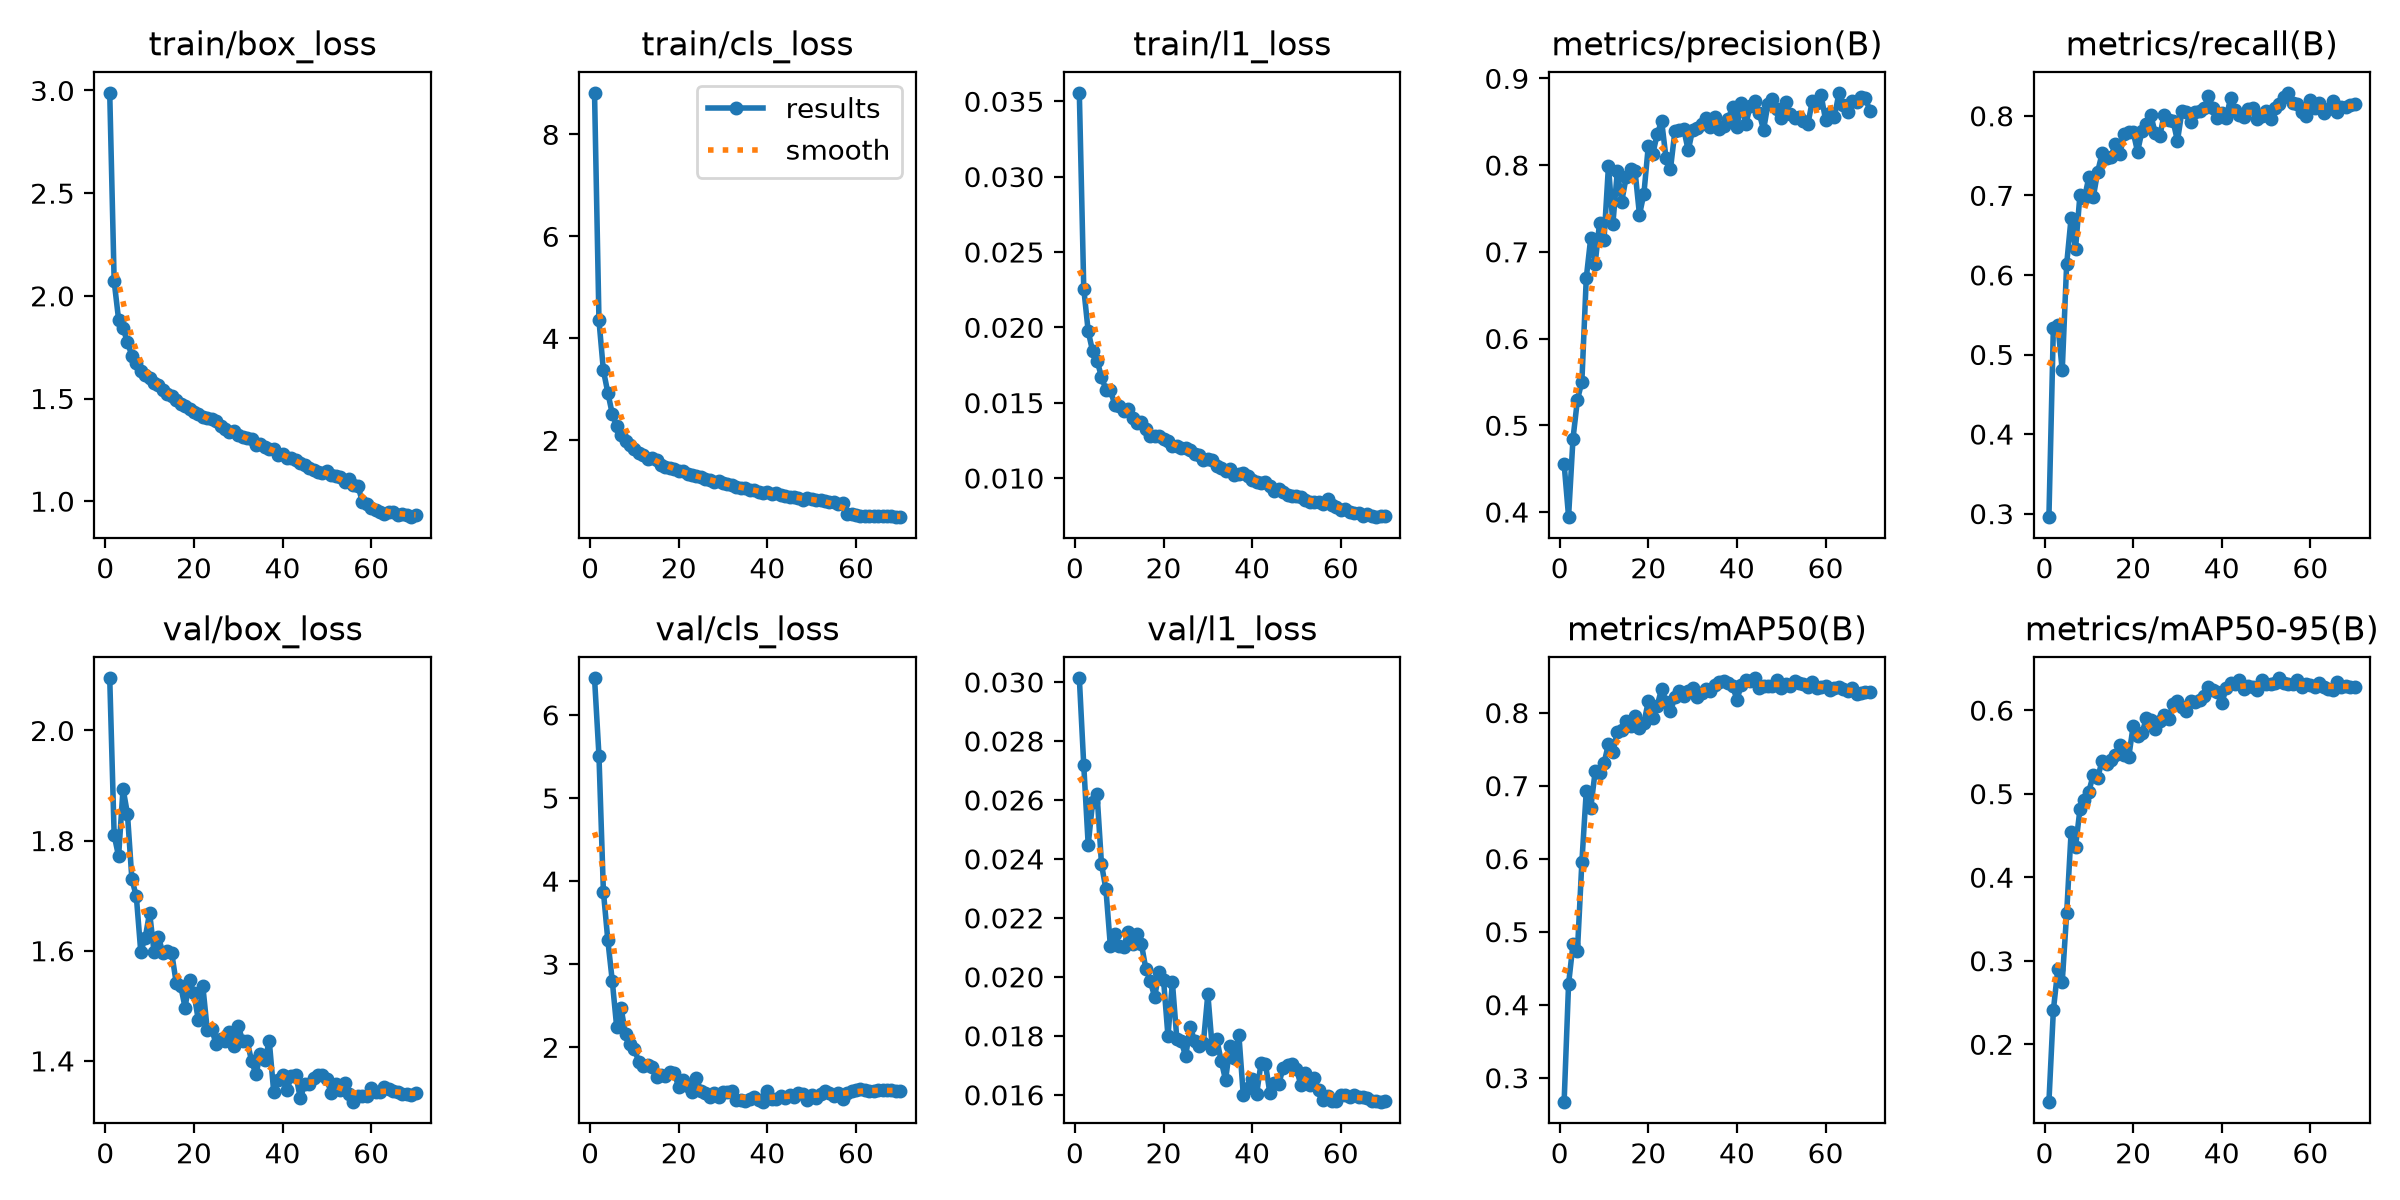
\includegraphics[width=\columnwidth]{yolo26n_p2_v13_results.png}
\caption{柑橘病蟲害偵測模型之訓練指標}
\end{figure}

圖2 為各類別的預測分布與混淆情形。在信心閾值 0.25 下，測試集 TP、FP、FN 為 675、118、135，Detection Jaccard 為 0.727；類別間誤判極少，漏檢多屬背景，以 Scale\_Insect（0.37）與 Citrus\_Leaf\_Miner（0.36）最高，顯示小目標與背景相似性仍是主要限制。本文方法九類測試 mAP50 為 0.86118，逐類結果見 4.5 節；Scale\_Insect 的 valid/test 差距為 0.1738，但相同資料三次訓練的差距介於 0.040 至 0.174，反映其評估集（各 35 張）過小。App 端 TFLite 模型因輸入固定為 640×640，測試 mAP50 為 0.857。

\begin{figure}[t]
\centering
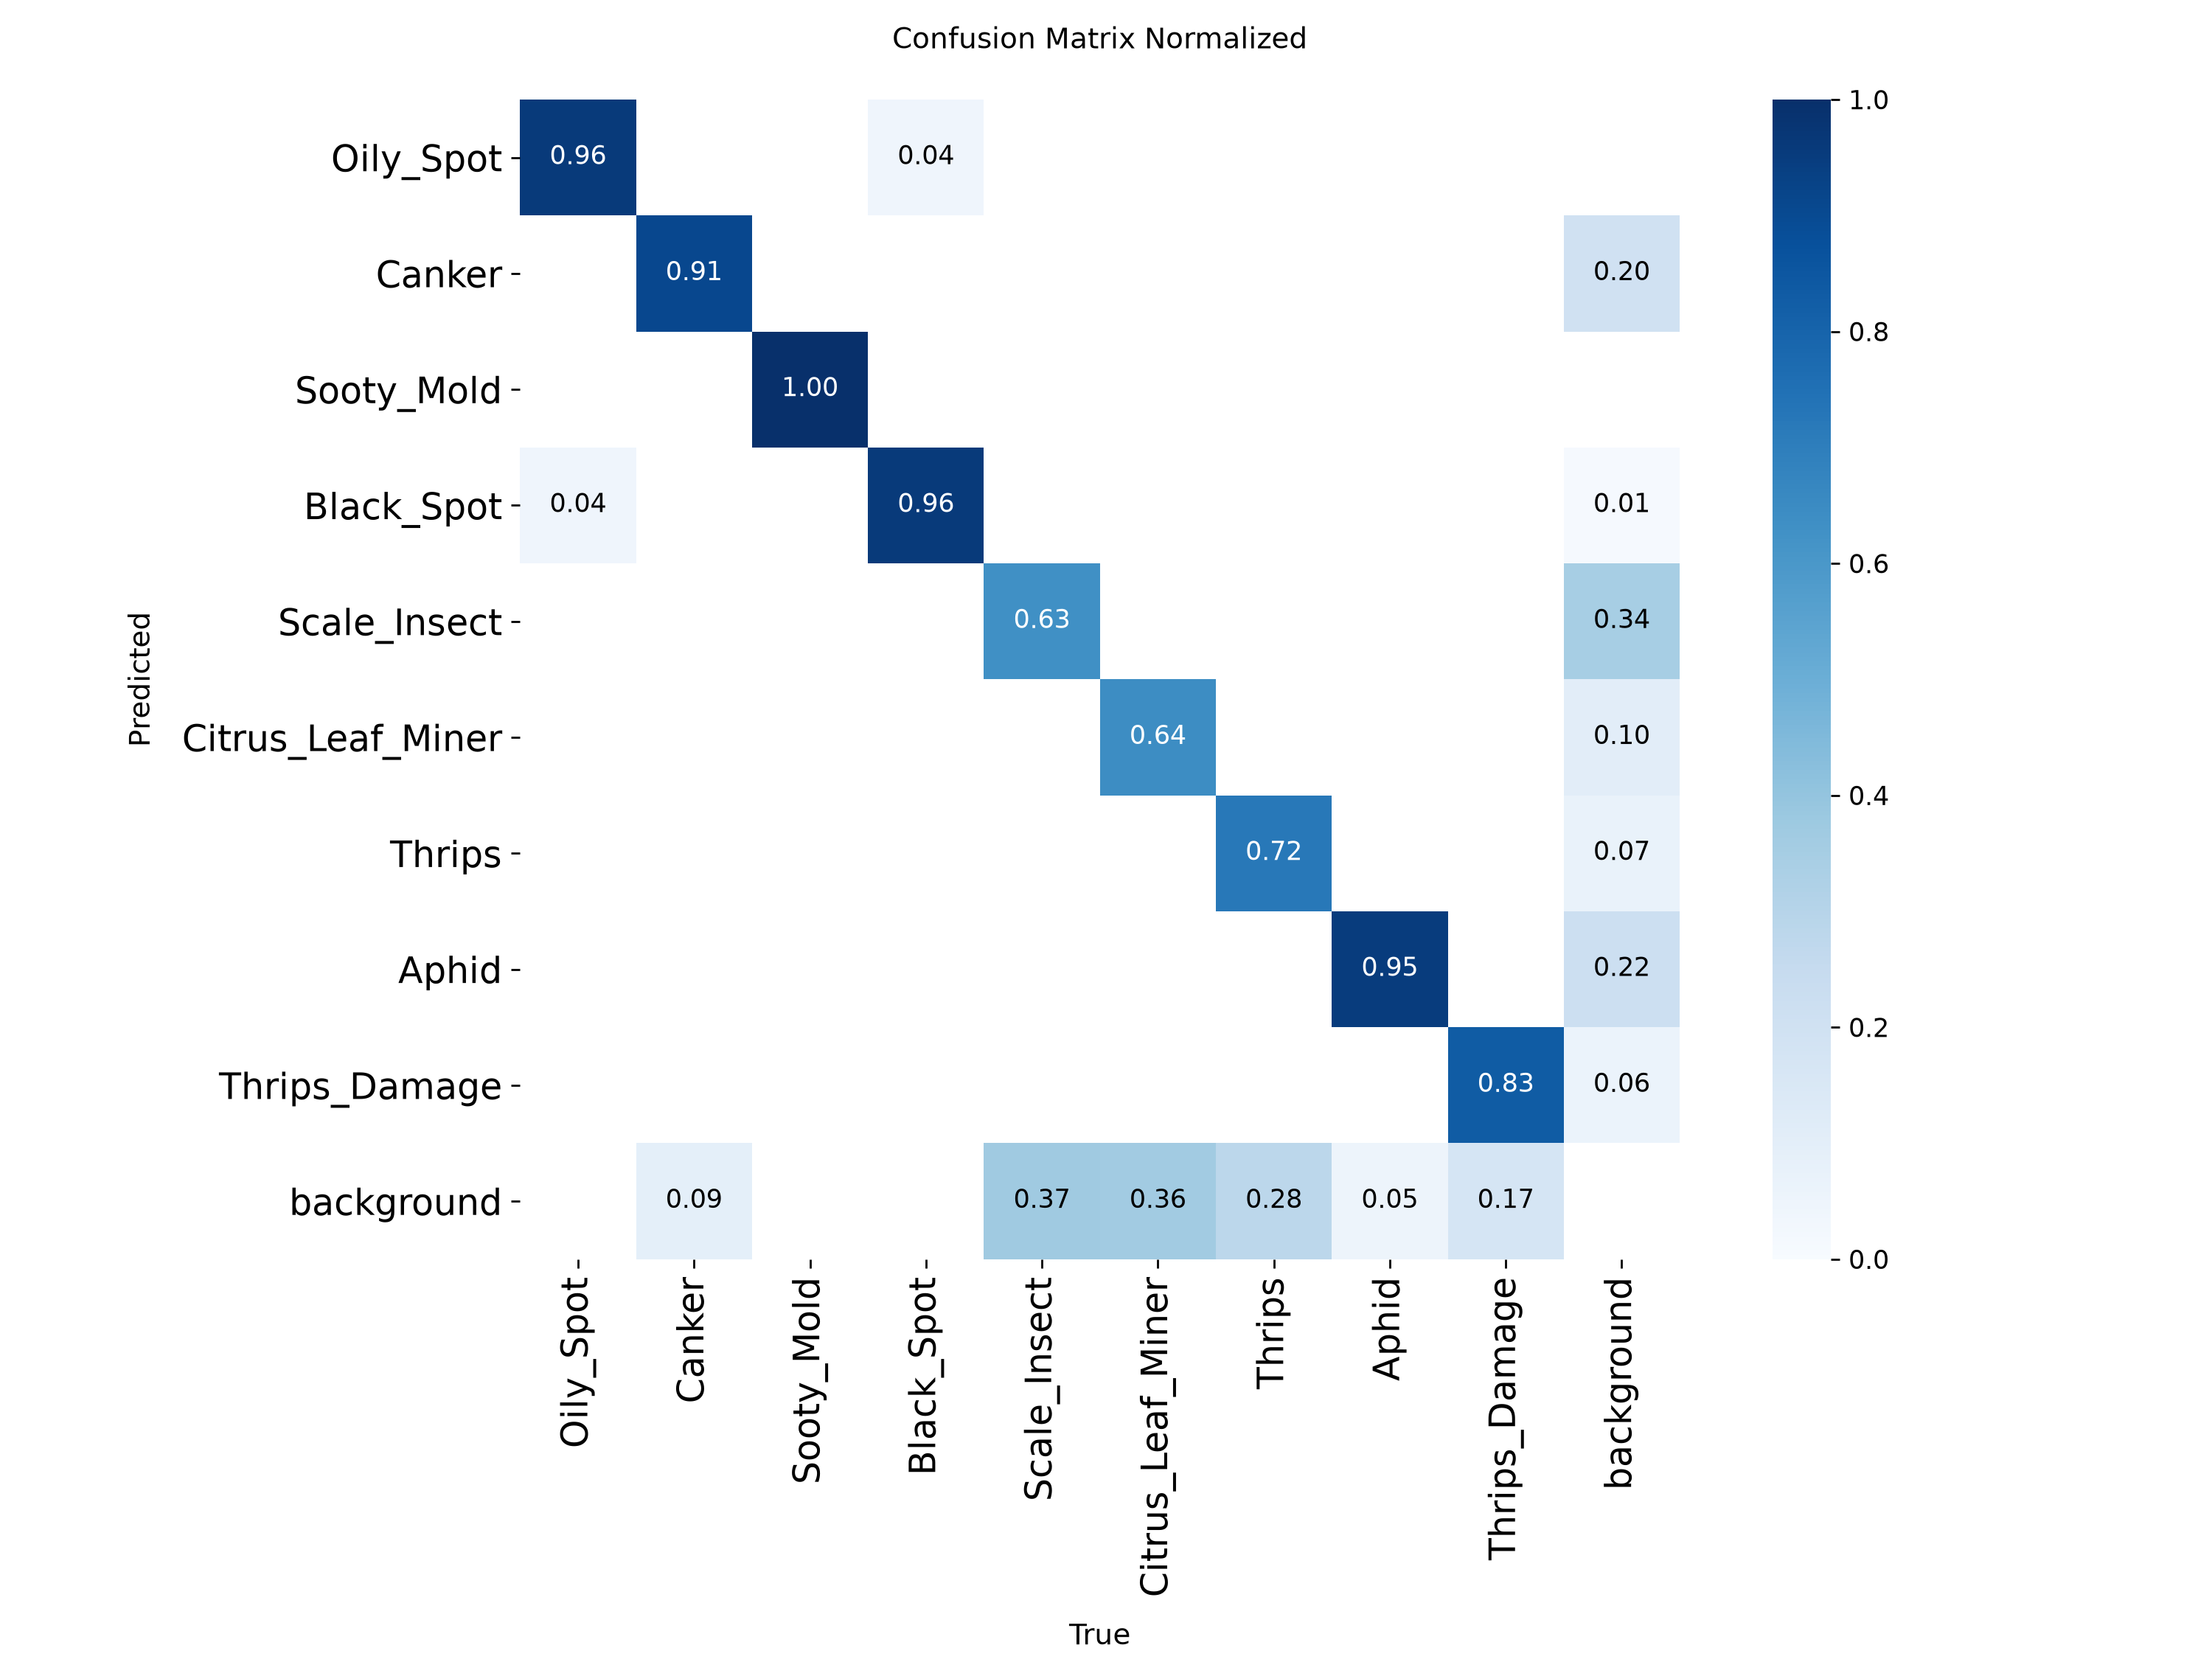
\includegraphics[width=\columnwidth]{yolo26n_p2_v13_confusion_matrix_norm.png}
\caption{測試集正規化混淆矩陣（信心閾值 0.25）}
\end{figure}

外部 detached-leaf 影像僅使 Citrus\_Leaf\_Miner 的 AP50 提升 0.0209，低於預設的 0.04 增益門檻，且與未加入資料的 Oily\_Spot（+0.0211）相當，表示資料領域不一致時，增加影像未必能改善田間辨識。九類 mAP50 較舊標註約定的 0.8096 高 0.0516，其中 0.0438 源自 Thrips\_Damage 標註框變大（中位面積由 11.30\% 增為 15.40\%）；未變動八類平均 AP50 為 0.8508，與舊約定的 0.8527 相近，故九類分數的變化不能直接解讀為模型能力全面提升。

\subsection{接地式診斷結果}
% 來源：20260924_citrus_rag_ablation_study.md 表 3-1 階段 5
完整系統（原子切片、自適應檢索、微調與護欄皆啟用）在 40 題評估的 Faithfulness 為 85.05\%、Context Precision 為 100.0\%、Context Recall 為 93.06\%，四題邊界題均成功防禦；Context Recall 未達 100\%，表示檢索仍可能遺漏部分答案條件。

典型錯誤包括偽造病原學名、混淆不同病蟲害的施用禁忌，以及將柑橘建議套用於非柑橘作物。原子切片與答案格式可減少前兩類錯誤；安全護欄則在跨作物、非農業提問或檢索為空時拒答。關閉護欄時，微調後模型對四題邊界題皆未能防禦，未微調模型亦僅防禦兩題，顯示安全性是模型、檢索與應用程式共同構成的系統性質。

\subsection{LLM+RAG 消融實驗}
% 來源：20260924_citrus_rag_ablation_study.md 表 3-1、§4.1–4.4（Galaxy A33、4 執行緒、Qwen2.5-7B 裁判 T=0.0）
表1 為五階段累加式消融結果，其中知識解耦貢獻最大：階段 1 的 10 筆粗粒度切塊使 0.5B 模型陷入重複輸出，平均輸出達 419.7 tokens；改用 33 筆原子切片後，Faithfulness 由 22.92\% 升至 83.86\%，輸出降至 73.6 tokens。參考 Pocket RAG \cite{kang2026} 的自適應檢索使 Context Precision 由 98.61\% 升至 100.0\%，Context Recall 由 89.58\% 升至 93.06\%。

\begin{table}[t]
\centering
\setstretch{1}\footnotesize
\setlength{\tabcolsep}{3pt}
\begin{tabular}{|l|c|c|c|c|c|}
\hline
\textbf{階段} & \textbf{Faith.} & \textbf{CP} & \textbf{CR} & \textbf{防禦} & \textbf{總耗時} \\
\hline
1 基線 & 22.92 & 75.00 & 44.91 & 0 & 37.08 \\
\hline
2 +原子切片 & 83.86 & 98.61 & 89.58 & 0 & 21.55 \\
\hline
3 +自適應檢索 & 82.64 & 100.0 & 93.06 & 50 & 22.61 \\
\hline
4 +監督式微調 & 87.04 & 100.0 & 93.06 & 0 & 30.85 \\
\hline
5 +安全護欄 & 85.05 & 100.0 & 93.06 & 100 & 29.98 \\
\hline
\end{tabular}
\caption{端側 RAG 五階段累加式消融結果（Galaxy A33，40 題；總耗時單位為秒，其餘為 \%）}
\end{table}

監督式微調使 Faithfulness 由 82.64\% 升至 87.04\%，淨增益 4.40 個百分點，PREP 結構遵從率由 15.00\% 升至 22.50\%；輸出由 90.0 增為 163.2 tokens，總耗時隨之增加，解碼速率則由 9.66 降為 9.40 tok/s，顯示微調主要改善證據依從與處方完整度，而非原生解碼能力。然而，微調也使模型以柑橘知識回答跨作物與非農業問題，無護欄時防禦率由 50\% 降為 0\%，加入護欄後達 100\%。階段 5 的 Faithfulness 較階段 4 低 1.99 個百分點；因各階段僅實測一次，尚不足以推論護欄會降低忠實度。

\subsection{行動端效能與限制}
% 來源：ablation study 表 3-1；20260729_mobile_rag_benchmark.md §2；detection docs/v13_報告 §4、v5.7_報告 §3.4
Galaxy A33 以 4 執行緒執行 40 題評估時，平均 TTFT 為 13.75 s，解碼速率 9.56 tok/s，單題總耗時 29.98 s。早期原型的純 SLM 測試中，6 執行緒可使 TTFT 由 2,613.1 ms 降至 2,110.3 ms、解碼速率由 10.40 升至 13.70 tok/s，但交付版本為兼顧功耗與溫控仍採 4 執行緒。持續影像推論在 Dimensity 8300 以 320 像素達 38.4 FPS，在 Snapdragon 8 Gen 2 達 29.8 FPS，Snapdragon 662 未通過準確度與延遲雙重門檻；這些量測使用架構相同的前一版權重，延遲可沿用，準確度須以交付權重重新評估。故目前採拍照後辨識，即時串流列為未來功能。

限制包括：偵測實驗各僅一個 random seed、標註一致性研究僅 20 張影像、RAG 消融各階段僅於單一手機實測一次、偵測與問答模組尚未整合評估，以及化學處置文字待專家與正式用藥標示核對。

\subsection{類別級結果與資料品質}
% 來源：detection docs/v5.7_報告 §3.1 第 1 點
為避免整體 mAP 掩蓋類別差異，本研究回報九類 pooled AP50。視覺特徵較集中的 Sooty\_Mold、Black\_Spot 與 Oily\_Spot 分別達 0.9950、0.9528 與 0.9482，Aphid 與 Canker 為 0.9297 與 0.9045；Thrips\_Damage、Citrus\_Leaf\_Miner、Thrips 與 Scale\_Insect 分別為 0.7848、0.7403、0.7040 與 0.6321。後四類存在小目標、遮蔽、形態變異或背景相似等問題，後續應優先補充不同生長期與拍攝距離的樣本。

資料驗收涵蓋影像與標註配對、類別編號、座標界限、資料洩漏、近重複影像跨子集、增強框面積比例與評估集絕對數量。九類 pooled 的 two-standard-error 上界均不超過 0.10，最大值為 Citrus\_Leaf\_Miner 的 0.099。這些檢查雖不能取代多次訓練，但有助於區分資料品質問題與模型隨機波動。標註一致性由 0.746 升至 0.899，亦說明影像任務的評估單位須先由領域知識定義清楚；全類重標後的實際一致性則為 0.80 至 0.83。

\subsection{問答評估與錯誤分析}
% 來源：ablation study §2.5–2.6；citrus-ragas-eval docs/academic_ragas_evaluation_methodology.md
Pilot 評估用於發現 prompt echoing、偽造學名、跨作物幻覺與回答格式問題；Full Benchmark 則以 36 題柑橘領域題及 4 題邊界題檢驗正式系統。評分以手機外的 Qwen2.5-7B-Instruct 為裁判（溫度 0）：先將答案拆為原子陳述，再依檢索內容判定是否受支持，切片未記載的藥劑、倍數或病徵皆視為不受支持\cite{es2023}。Faithfulness 為受支持陳述比例，Context Precision 衡量第一順位切片是否相關，Context Recall 衡量參考答案所需資訊是否被涵蓋；此設計比字串完全比對更適合結構化農業回答。

錯誤分析顯示，偵測正確不代表診斷文字安全。病原、藥劑與作物名稱相近時，短 context 可能使模型錯誤合併兩個實體；使用者僅提供「葉子變黃」等低資訊問題時，模型也可能給出超出證據的處置建議。因此回答須同時呈現辨識結果、檢索依據與未驗證狀態，並保留人工覆核機制；化學用藥不應由模型自行推論，應轉介正式標示或農業專家。

\subsection{端側處理流程與工程取捨}
% 來源：citrus-rag-mobile rag_orchestrator_service.dart；report RAG向量資料庫/架構設計.md §1、§6.3；ablation study §3.2
系統流程分為影像輸入、候選偵測、使用者追問、安全檢查、知識檢索與答案生成六個步驟，影像與問答資料皆於手機內處理。知識庫（約 30 KB）以 App 內建資產載入，379 MB 的模型權重則置於應用程式沙盒並以 mmap 載入，以降低記憶體壓力。檢索平均約 10.18 ms，僅占單題總耗時的 0.03\%，因此最佳化重點應為模型載入、prompt prefill、context 長度與答案快取。

在 Galaxy A33 上，TTFT 約占單題總耗時的 46\%，prompt prefill 為主要瓶頸；早期原型以 30 至 250 字短提示量測的 2,110.3 ms 屬於不同協定，兩者不應混為單一產品延遲。低階裝置較適合拍照後辨識而非持續串流；高階裝置亦應以持續負載而非單次峰值 FPS 作為部署依據。

\subsection{實驗控制與結果解讀}
本研究將資料品質、模型能力與應用效能分開控制。偵測實驗固定資料切分與輸入尺寸，並同時報告九類與未變動八類結果，避免因單一類別的框選規則改變而誤判模型全面提升。外部影像實驗固定訓練影像總數，僅改變部分影像來源與背景，以判斷增益來自樣本數或領域相似性；結果顯示白紙背景的 detached-leaf 影像無法直接取代果園影像。

各偵測指標的定義亦須區分：mAP50 為 IoU=0.5 下的平均精確度均值，mAP50–95 對定位更嚴格；Precision 反映誤報，Recall 反映漏報，混淆矩陣的 Jaccard 則以固定信心閾值計算，不應在同一表格中視為同義。對農業使用者而言，低 Recall 可能遺漏小型害蟲，低 Precision 則可能造成不必要的人工檢查，因此部署時應依使用情境調整閾值，而非追求單一最高分。

問答評估亦分層解讀：同時報告 Faithfulness、Context Precision 與 Context Recall，可區分「檢索正確但回答越界」、「檢索遺漏」與「模型未依從證據」三類失效；邊界題檢驗系統能否在證據不足時停止生成，為農業處置情境不可省略的安全指標。

\subsection{使用情境與風險管理}
% 來源：OneLeaf-dx/APP README.md（功能與架構）；citrus-rag-mobile rag_orchestrator_service.dart（0-Hit 回覆）
使用者拍攝葉片或自相簿選取影像後，系統回傳候選病蟲害、信心分數與 bounding box，並以信心最高的候選結果開啟問答，使用者可再輸入症狀或管理問題。端側檢索依作物、病蟲害、病徵與問題詞彙選擇切片；若無切片通過門檻，系統顯示查無高信心知識並建議諮詢在地專家，而非以一般語言模型知識作為正式防治建議。回答中應保留證據摘要，以利使用者追溯建議來源。

風險管理分為三層：資料層將不同作物、病蟲害與施用條件分開建檔，以免切片互相污染；模型層以微調與結構化輸出減少偽學名、重複語句與跨實體混淆；應用層在檢索結果為空、跨作物或非農業提問時中止，化學名稱與未驗證處置的標註則列為後續工作。三層機制缺一不可，因為再完善的模型仍可能遭遇資料庫未涵蓋的新情境。

本系統定位為離線的初步篩檢與證據導覽工具，而非自動開立處方。農民可依辨識結果決定是否補拍其他角度或尋求專業協助；農業人員可利用 bounding box、候選類別與來源切片加速初步判讀。正式用藥仍須核對農業部\cite{moa2026} 公告、產品標示、適用作物與病蟲害範圍，以及施用濃度與安全採收期。

\subsection{可重現性與後續研究}
為確保可重現性，本研究記錄資料集切分、影像與標註數量、標註規則、近重複檢查方法、模型訓練設定、信心閾值、知識切片版本、題庫內容、評分裁判規則、裝置型號與執行緒數。每次更新資料或知識庫後，應重新執行洩漏檢查、類別級評估、邊界題與長時間負載測試；若僅更新模型權重而未重新驗證知識庫，無法確保問答安全性，僅更新知識庫也可能改變答案分布與延遲。

後續研究有四個方向：（1）偵測與 RAG 實驗皆重複至少三次並擴及多種手機與作物，報告平均值與 bootstrap 信賴區間；（2）將標註一致性研究擴大至九類、不同拍攝條件與病徵嚴重度；（3）蒐集與訓練資料同領域的果園影像，以 farm-level split 評估跨果園泛化；（4）由兩位農業專家審查所有化學處置陳述，分別報告模型忠實度與實務正確性。這些工作可將工程驗證推進至田間部署驗證。

\section{結論}
本研究提出完全於端側執行的柑橘病蟲害辨識與接地式診斷方法。偵測模型於九類測試集的 mAP50 為 0.861、mAP50–95 為 0.641；端側 RAG 於 40 題評估達 Faithfulness 85.05\%、Context Precision 100.0\% 與 Context Recall 93.06\%，並能防禦跨作物與領域外邊界問題。消融實驗顯示知識切片粒度影響最大，且微調模型須搭配護欄。整體結果顯示，資料標註一致性、領域相似性、檢索證據與安全護欄對系統可靠性的影響不亞於模型架構。此方法可作為離線農業輔助工具的基礎，但防治建議仍應以官方標示與農業專業人員判斷為準。

\section{誌謝}
本研究部分經費由國家科學及技術委員會補助（NSTC 115-2221-E-025-006），謹此致謝。

% 參考文獻依原版的引用順序編號（IEEE 格式）；作者、卷期與頁碼已逐筆查核，見〈論文修訂說明〉§8
\begin{thebibliography}{23}
\bibitem{mohanty2016} S. P. Mohanty, D. P. Hughes, and M. Salathé, ``Using deep learning for image-based plant disease detection,'' \textit{Frontiers in Plant Science}, vol. 7, p. 1419, 2016.
\bibitem{ferentinos2018} K. P. Ferentinos, ``Deep learning models for plant disease detection and diagnosis,'' \textit{Computers and Electronics in Agriculture}, vol. 145, pp. 311--318, 2018.
\bibitem{kamilaris2018} A. Kamilaris and F. X. Prenafeta-Boldú, ``Deep learning in agriculture: A survey,'' \textit{Computers and Electronics in Agriculture}, vol. 147, pp. 70--90, 2018.
\bibitem{pacal2024} I. Pacal, I. Kunduracioglu, M. H. Alma, M. Deveci, S. Kadry, J. Nedoma, V. Slany, and R. Martinek, ``A systematic review of deep learning techniques for plant diseases,'' \textit{Artificial Intelligence Review}, vol. 57, no. 11, p. 304, 2024.
\bibitem{moa2026} Ministry of Agriculture, Taiwan, ``Ministry of agriculture official website,'' [Online]. Available: \url{https://www.moa.gov.tw/}, 2026. Accessed: 2026-07-02.
\bibitem{hughes2015} D. P. Hughes and M. Salathé, ``An open access repository of images on plant health to enable the development of mobile disease diagnostics,'' arXiv preprint arXiv:1511.08060, 2015.
\bibitem{guan2023} H. Guan, C. Fu, G. Zhang, K. Li, P. Wang, and Z. Zhu, ``A lightweight model for efficient identification of plant diseases and pests based on deep learning,'' \textit{Frontiers in Plant Science}, vol. 14, p. 1227011, 2023.
\bibitem{xiong2024} H. Xiong, J. Li, T. Wang, F. Zhang, and Z. Wang, ``EResNet-SVM: An overfitting-relieved deep learning model for recognition of plant diseases and pests,'' \textit{Journal of the Science of Food and Agriculture}, vol. 104, no. 10, pp. 6018--6034, 2024.
\bibitem{ashurov2025} A. Y. Ashurov, M. S. A. M. Al-Gaashani, N. A. Samee, R. Alkanhel, G. Atteia, H. A. Abdallah, and M. Saleh Ali Muthanna, ``Enhancing plant disease detection through deep learning: A depthwise CNN with squeeze and excitation integration and residual skip connections,'' \textit{Frontiers in Plant Science}, vol. 15, p. 1505857, 2025.
\bibitem{xu2023} Y. Xu, Z. Gao, Y. Zhai, Q. Wang, Z. Gao, Z. Xu, and Y. Zhou, ``A CNNA-based lightweight multi-scale tomato pest and disease classification method,'' \textit{Sustainability}, vol. 15, no. 11, p. 8813, 2023.
\bibitem{goyal2025} A. Goyal and K. Lakhwani, ``Integrating advanced deep learning techniques for enhanced detection and classification of citrus leaf and fruit diseases,'' \textit{Scientific Reports}, vol. 15, p. 12659, 2025.
\bibitem{he2016} K. He, X. Zhang, S. Ren, and J. Sun, ``Deep residual learning for image recognition,'' in \textit{Proc. CVPR}, pp. 770--778, 2016.
\bibitem{deng2009} J. Deng, W. Dong, R. Socher, L.-J. Li, K. Li, and L. Fei-Fei, ``ImageNet: A large-scale hierarchical image database,'' in \textit{Proc. CVPR}, pp. 248--255, 2009.
\bibitem{lin2017} T.-Y. Lin, P. Goyal, R. Girshick, K. He, and P. Dollár, ``Focal loss for dense object detection,'' in \textit{Proc. ICCV}, pp. 2980--2988, 2017.
\bibitem{selvaraju2017} R. R. Selvaraju, M. Cogswell, A. Das, R. Vedantam, D. Parikh, and D. Batra, ``Grad-CAM: Visual explanations from deep networks via gradient-based localization,'' in \textit{Proc. ICCV}, pp. 618--626, 2017.
\bibitem{shorten2019} C. Shorten and T. M. Khoshgoftaar, ``A survey on image data augmentation for deep learning,'' \textit{Journal of Big Data}, vol. 6, no. 1, p. 60, 2019.
\bibitem{feng2025} W. Feng, J. Liu, Z. Li, and S. Lyu, ``YOLO-Citrus: A lightweight and efficient model for citrus leaf disease detection in complex agricultural environments,'' \textit{Frontiers in Plant Science}, vol. 16, p. 1668036, 2025, doi: 10.3389/fpls.2025.1668036.
\bibitem{hu2021} E. J. Hu, Y. Shen, P. Wallis, Z. Allen-Zhu, Y. Li, S. Wang, L. Wang, and W. Chen, ``LoRA: Low-rank adaptation of large language models,'' arXiv preprint arXiv:2106.09685, 2021.
\bibitem{qwen2025} Qwen Team, ``Qwen2.5 technical report,'' arXiv preprint arXiv:2412.15115, 2025.
\bibitem{kang2026} D. H. Kang, H. Lee, H. Cha, M. Choi, and S. Lim, ``Pocket RAG: On-device RAG for first aid guidance in offline mobile environment,'' arXiv preprint arXiv:2602.13229, 2026.
\bibitem{guainazzo2026} N. Guainazzo, G. Delzanno, D. Ancona, and D. D'Agostino, ``Navigating the Seas of AI: Effectiveness of small language models on edge devices for maritime applications,'' \textit{Sensors}, vol. 26, no. 5, p. 1590, 2026, doi: 10.3390/s26051590.
\bibitem{rafailov2023} R. Rafailov, A. Sharma, E. Mitchell, C. D. Manning, S. Ermon, and C. Finn, ``Direct preference optimization: Your language model is secretly a reward model,'' in \textit{Advances in Neural Information Processing Systems}, vol. 36, pp. 53728--53741, 2023.
\bibitem{es2023} S. Es, J. James, L. Espinosa-Anke, and S. Schockaert, ``RAGAS: Automated evaluation of retrieval augmented generation,'' arXiv preprint arXiv:2309.15217, 2023.
\end{thebibliography}

\end{document}
